\documentclass[a4paper]{article}
\usepackage[latin1]{inputenc}
\usepackage{graphicx}
\usepackage{array}
\usepackage{amsmath}
\newcommand{\transp}{\top}

\usepackage{caption}
\usepackage{subcaption}

\setlength{\parskip}{2ex}

\begin{document}


\title{Deep Q-Learning Report}
\author{Francisco Garcia, Ian Gemp, Kevin Spiteri, Nabanita De}
%\date{}

\maketitle


For this project, we studied the behavior of DeepMind's Deep Q-Learning work on two Atari domains: Pong and Boxing.
We let the agents train for 40 epochs and observed the returns as well as their behavior. The plots of training on each game are shown in Figure 1.
From these graphs, we can observe that the agent for Pong quickly learns a policy that consistently gives positive returns, i.e. learns a strategy to beat its opponent. However, the plot corresponding to boxing shows that the agent is unable to find a winning strategy.
By carefully looking at the characteristics that differentiate these games and taking into account how the learning network is set up, we were able to identify several possibilities that would make boxing that much harder to learn.

\begin{itemize}
\item \textbf{Number of available actions:} An obvious difference is the number of available actions in each game. Pong limits actions to 3 (move up, move down or stay in the same position), whereas in Boxing there are 6 possible actions (up, down, left, right, stay and punch)

\item \textbf{Role of adversary:} A clear distinction in the games is the role the adversary plays in a winning strategy. In Pong, the adversary is irrelevant, as long as the paddle of our agent is in the right position to prevent the opponent from scoring, it will never lose and the opponent cannot do anything about it.Eventually, our agent will be able to score. On the other hand, our opponent plays a more significant role in Boxing. There is no safe strategy for not losing, since our opponent is able to reach our position and score.  

\item \textbf{Predictability of the game:} Another important difference, in our opinion, is how predictable the game is based on the last four frames (DeepMind's network keeps track of a history of four frames). In the case of Pong, if you look at the last for frames, not only are you able to determine in which direction the ball is heading, but you can determine exactly where the ball is going to be by the time it reaches one of the paddles, since it moves in a straight line and bounces off the walls maintaining the same x,y speed. However, in the case of Boxing, the last four frames doesn't say much about which direction the opponent will move next. For example, if in the last four frame the opponent was moving in the positive x-direction, the next frame it might choose to move either up, down, left, right or not move. This difference is also related to the role the opponent plays in the game. As mentioned before, the position of the opponent is irrelevant in Pong to find a non-losing strategy, but this is not true in the case of Boxing.

\end{itemize} 

 
 We suspect that given these characteristics of Boxing, we might not have trained the network long enough to build an efficient agent. It is hard to tell whether the networks used for reporting results were fined tuned for each game or they simply present a different level of difficulty for a learning agent. 
 
\begin{figure}
\centering
\begin{subfigure}{.5\textwidth}
  \centering
  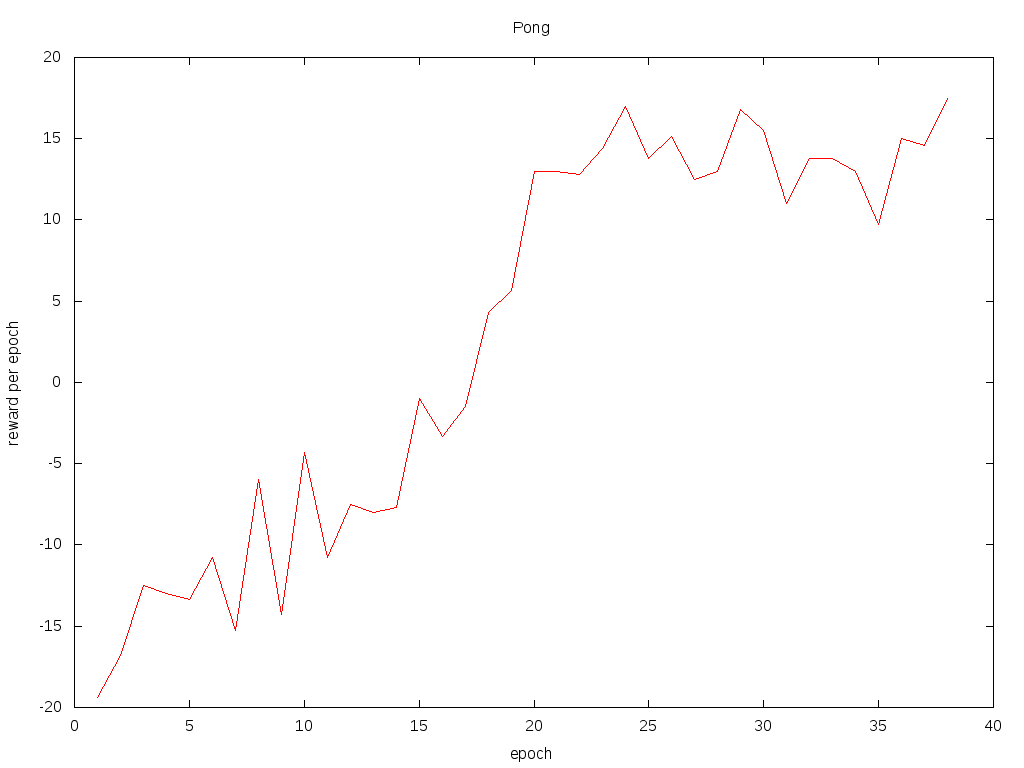
\includegraphics[width=.8\linewidth]{pong.png}
  \caption{DMP for joint 1}
  \label{fig:sub1}
\end{subfigure}%
\begin{subfigure}{.5\textwidth}
  \centering
  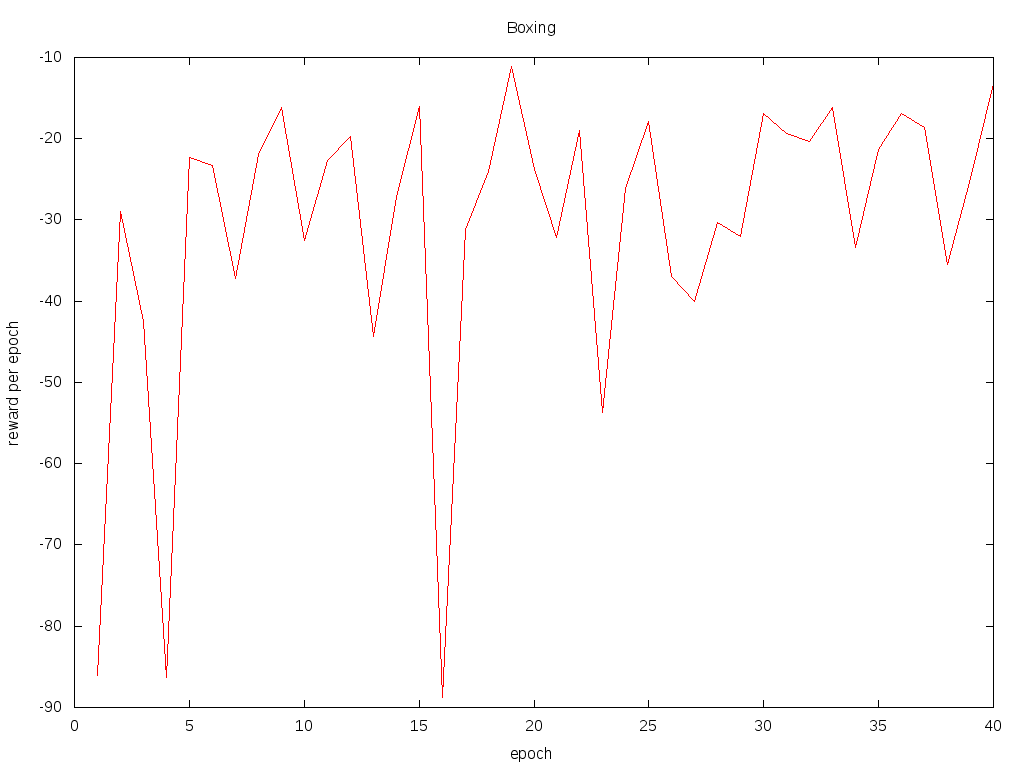
\includegraphics[width=.8\linewidth]{boxing.png}
  \caption{DMP for joint 2}
  \label{fig:sub2}
\end{subfigure}
\caption{Plot of demonstrations and their corresponding DMP}
\label{fig:test}
\end{figure}


  
\end{document}